\chapter{Ray tracing on phase space} \label{chap:PS}
Ray tracing on phase space is method which employs the phase space (PS) of the source and the target of the optical systems. 
It takes into account of the trajectory that every ray follows during its propagation.
We show through this chapter that this allows to trace only the rays close to the discontinuity of the luminance.
Before explaining the method, we need to introduce the PS concept.
\section{Phase space concept}
The PS of a three-dimensional systems is a four-dimensional space since every ray is described by two position coordinates
and two direction coordinates.
The two position coordinates are given by two of the coordinates of the intersection point of the ray with the surface, while the two direction coordinates are
the momentum coordinates of the vector tangent to the ray projected on the optical surface, see \cite{wolf2004geometric}.
\\ \indent For two-dimensional systems every ray in the PS of a line is given by a point in a two-dimensional space.
The position coordinate in the PS of line $\lineai$ is the \variabile{x}-coordinate of the intersection point between the ray and line $\lineai$.
The direction coordinate is the sine of the angle that the ray forms with respect to the normal of line $\lineai$ multiplied by the index of refraction of the medium in which the ray is located.
We indicate the PS with \set{S}{}{}$=$\set{Q}{}{}$\times$\set{P}{}{},
where \set{Q}{}{} is the set of the position coordinates \variabile{q} and \set{P}{}{} is the set of the direction coordinates $\variabile{p}=\variabile{n}\sin{\myangle}$ with $\myangle$ the angle between the ray and the normal \vect{$\boldsymbol{\nu}$} of the line and \variabile{n} is the index of refraction of the medium in which the line is located.  
The normal \vect{$\boldsymbol{\nu}$} is always directed inside the same medium in which the incident ray travels and, 
the angle $\myangle$ between the ray and \vect{$\boldsymbol{\nu}$} is measured counterclockwise.
In the following, the phase space is considered only for the source $\point{S}$ and the target $\point{T}$ and for no other line of the optical system.
The coordinates of every ray on \set{S}{}{} and \set{T}{}{} are indicated with $(\variabile{q}_1,\variabile{p}_1)$ and $(\variabile{q},\variabile{p})$, respectively. 
\begin{figure}[h]
  \begin{minipage}[h]{0.5\textwidth}
    \includegraphics[width=\textwidth]{source_PS_cup.pdf}
    \caption{Source PS of the two-faceted cup.}
    \label{fig:coefficients}
  \end{minipage} 
  \begin{minipage}[h]{0.5\textwidth}
    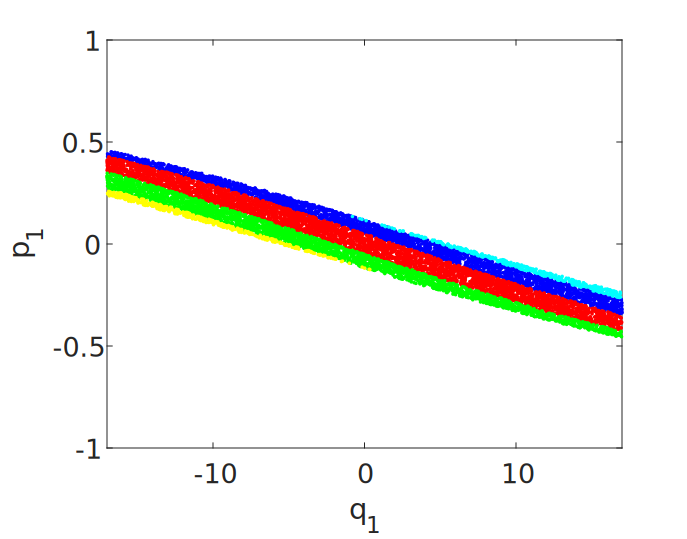
\includegraphics[width=\textwidth]{target_PS_cup.pdf}
    \caption{}
   \label{fig:coefficients2}
 \end{minipage}
\end{figure}


% Show source and target PS
% In fig. \ref{fig:sourcePS} and \ref{fig:targetPS} we show the source and target PS distribution of rays
\\ \indent The source and target phase spaces are partitioned into different regions according to the path $\Pi$ followed by the rays. 
Given a path $\Pi$, the corresponding regions are indicated with \set{R}{$1$}{}$(\Pi)$ and \set{R}{}{}$(\Pi)$ at the source and the target PS, respectively. 
A map $\map{M}{}{}$:\set{S}{}{}$\rightarrow$\set{R}{}{}$(\Pi)\subseteq$\set{T}{}{} which describes how the optical system changes the rays is defined as:
\begin{equation}\label{M}
\map{M}{}{}(\variabile{q}_1,\variabile{p}_1)=(\variabile{q}, \variabile{p}).
\end{equation} 
For very simple systems, as for example the two-faceted cup, it is possible to determine an analytic expression for $\map{M}{}{}$.
This is not the case of most of the optical systems we deal with. 
We can in that case use the edge ray principle, \cite{welford1978problem}.
Ries and Rabl (1994) showed that the boundaries 
$\partial$\set{R}{$1$}{}$(\Pi)$ at the source are mapped into the boundaries $\partial$\set{R}{}{}$(\Pi)$ at the target: all rays that are neighbors at the source PS remain close to each other at the target PS, \cite{Ries:2}. Then, to map one region from the \set{S}{}{} to \set{T}{}{} it is sufficient to map the boundary of this region.
% Say that this is an extended version of the edge-ray principle.
\\ \indent Using the PS concept and the edge-ray principle we develop a new ray-tracing procedure in PS.
\section{Phase space ray tracing}
 
The regions $(R_{\textrm{t}, \Pi_j})_{j =1, \cdots, p}$ can be defined only when some rays are traced.
Given an initial set of rays, the rays closest to the boundaries $(\partial R_{\textrm{t}, \Pi_j})_{j = 1, \cdots, p}$ are selected and more rays in their vicinity are created to get progressively better estimates of the boundaries. A more detailed description is provided below.
A triangulation in $\mathcal{P}_\textrm{s}$ is defined and a ray from every vertex $(x_k, \tau_k)$ of the triangle is traced.
The procedure starts tracing four rays with coordinates $(x_k,\tau_k)_{k=1, \cdots, 4}$ that are located exactly at the corners of $\mathcal{P}_\textrm{s}$ and, for each of them, the paths $(\Pi_{j})_{j = 1, \cdots, 4}$, are stored. Next, for some $j \in\{1, \cdots, 4\}$, the grid is divided into two equal triangles joining two opposite vertices. For each triangle the rays located at its corners are traced. If the paths corresponding to
those rays are different, one or more boundaries
$(\partial R_{\textrm{t}, \Pi_j})_{j =1, \cdots, 4}$ are expected to cross the triangle.
In that case, the middle points $(x_k, \tau_k)_{k = 5, 6, 7}$ of each side of the triangle are added and
three more rays with coordinates $(x_k, \tau_k)_{k = 5, 6,7}$ are traced. Each refinement step leads to four new triangles (see Figure \ref{fig:refinement}).
 \begin{figure}[h]
  \begin{center}
  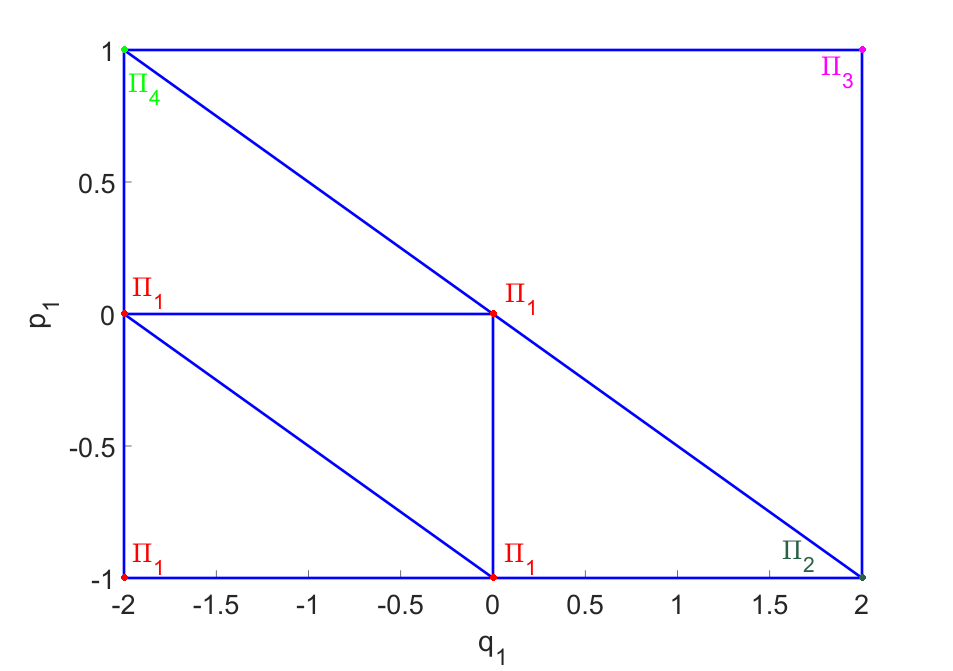
\includegraphics[width=8cm]{region}
  \end{center}
  \caption{Triangulation refinement:
  when the rays related to the vertices of the triangles follow a different path a new refinement step is required.
   Each refinement step leads to four new triangles.
   The parameters values are $\epsilon_{x_{max}}~=~ 2$, $\epsilon_{\tau_{max}}= 1$, $\epsilon_{x_{min}}= 4$ and $\epsilon_{\tau_{min}}=2$.}
  \label{fig:refinement}
\end{figure}
  \\
 \indent
When all the rays in the corners of each triangle have the same path, it is not necessary to refine the triangles anymore.
\noindent Note that it can happen that a region formed by rays that follow a path $\Pi_j$ is located completely inside a triangle whose vertices are related to the same path $\Pi_i$ with $j \neq i$. In that case the algorithm is not able to detect that region, see Figure \ref{fig:region inside}. To avoid this, two parameters $\epsilon_{x_{min}}$ and $\epsilon_{\tau_{min}}$ are defined for the $x$-axis and the $\tau$-axis, respectively. When the length of the sides of the triangle are greater than these parameters, a new triangle is defined even if its vertices correspond to the same path. Furthermore, two other parameters $\epsilon_{x_{max}}$ and $\epsilon_{\tau_{max}}$ are introduced to defined a stopping criterion.
The algorithm stops when the length of the sides of the triangles is smaller than $\epsilon_{x_{max}}$ and $\epsilon_{\tau_{max}}$.
\begin{figure}[h]
  \begin{center}
  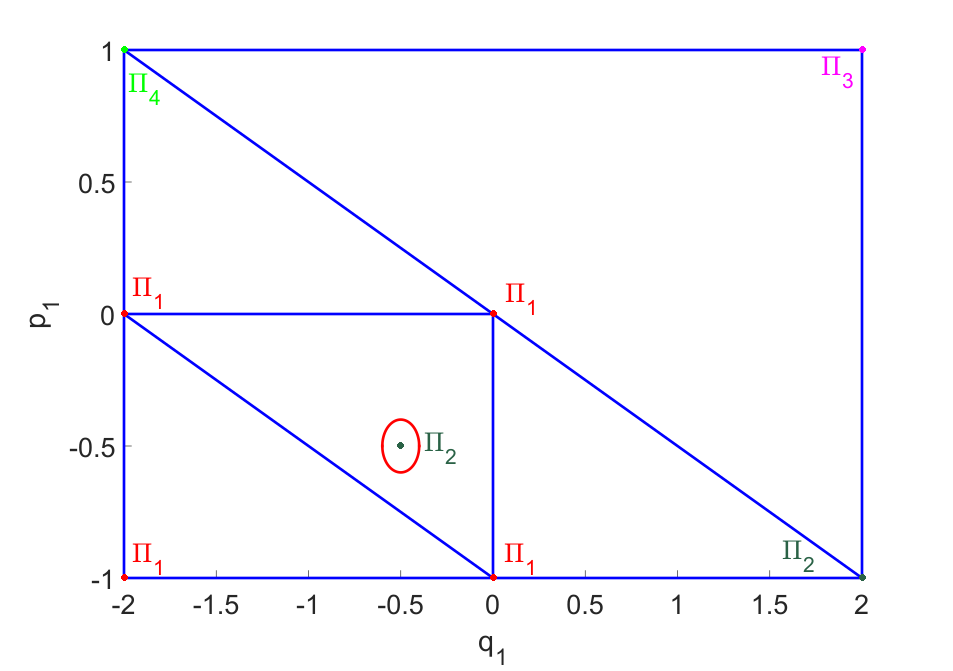
\includegraphics[width=8cm]{region_inside}
  \end{center}
  \caption{The red line encloses a region of rays that follow the path $\Pi_2$ and is completely located inside a triangle.
  The algorithm is not able to detect that region and, a further refinement is required.
    The parameters values are $\epsilon_{x_{max}}~=~ 2$, $\epsilon_{\tau_{max}}= 1$, $\epsilon_{x_{min}}= 4$ and $\epsilon_{\tau_{min}}=2$. }
   \label{fig:region inside}
  \end{figure}
The values of the parameters $\epsilon_{x_{max}}$, $\epsilon_{\tau_{max}}$, $\epsilon_{x_{min}}$ and $\epsilon_{\tau_{min}}$ determine the number of rays traced.
Indeed, on the one hand, $\epsilon_{x_{max}}$ and $\epsilon_{\tau_{max}}$ can be decreased to obtain more rays close to the boundaries;
on the other hand, a large number of rays in the interior of the regions can be traced decreasing the values of $\epsilon_{x_{min}}$ and $\epsilon_{\tau_{min}}$. %
\newline
\indent Using the above procedure, rays increasingly closer to the boundaries are traced.
For our optical system, the width of the $x$-axis in source phase space is two times the width of the $\tau$-axis.
Thus, our choice is $\epsilon_{\tau_{min}}=\frac{1}{2}\epsilon_{x_{min}}$ and $\epsilon_{\tau_{max}} = \frac{1}{2}\epsilon_{x_{max}}$.
Figure \ref{fig:triangulation_refinement} shows an example of a triangulation refinement of the source phase space with $\epsilon_{x_{max}}=0.1$ and $\epsilon_{x_{min}}=1$.
The triangulation refinement provides more triangles close to the boundaries $\partial R_{\textrm{s}, \Pi_j}$ than those inside the regions $R_{\textrm{s}, \Pi_j}$.
\begin{figure}[h]
  \begin{center}
  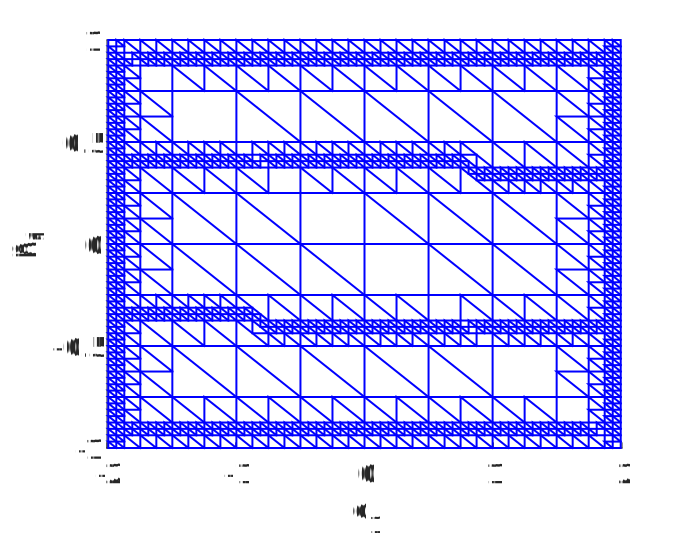
\includegraphics[width=8cm]{triangulation_source}
  \end{center}
  \caption{Triangulation refinement of source phase space:
  near the boundaries more rays are traced.
    The values of the parameters are $\epsilon_{x_{max}}~=~ 0.1$ and $\epsilon_{x_{min}}~=~1$.}
   \label{fig:triangulation_refinement}
  \end{figure}
 \\ \indent The paths $(\Pi_j)_{j = 1, \cdots, p}$ followed by the rays located at the corner of the triangles are computed during the procedure and, the regions
 $R_{\textrm{s}, \Pi_j}$ and $R_{\textrm{t}, \Pi_j}$ are defined for each $\Pi_j$.
Next, a criterion to select the values of the parameters $\epsilon_{x_{min}}$ and $\epsilon_{x_{max}}$ and a method to compute the boundaries $\partial{R_{t, \Pi_j}}$ is provided.
Furthermore, the output photometric variables are computed, the details are explained in the next section.



\section{Comparison between MC, QMC and PS ray tracing}

% Compare all the PS
% Definition of luminance intensity and etendue

\indent A similar method as described in this chapter is presented by Moore, \cite{moore2013methods}. In Moore's method each ray leaves the source at the same position while the angle coordinate changes. The path followed by the rays is taken into account and an interpolation is required to finalize the illumination pattern.
 This interpolation can affect the efficiency of the method. Our method employs the distribution of the rays at the target phase space and avoids using any interpolation. 
Moreover, a criterion to stop the algorithm is provided in such a way that no more rays than necessary are traced. This makes ray tracing in phase space more accurate compared with Moore's procedure.
 Finally, we claim that PS ray tracing is also more accurate than the ray tracing procedure proposed by Moore (2013), \cite{moore2013methods}.
The novelty of our approach compared to the method used by Moore, is briefly explained below.
First, to compute the output intensity, we employ the phase space of the target. This avoids the use of any interpolation to compute the photometric variables and therefore, more accurate results are obtained.
Second, in \cite{moore2013methods} all rays that leave the source start at the same position and only a sampling angular range is given. In our approach a rectangular source is considered thus, both the angular and spatial coordinates of each ray change. This extra variable can produce very irregular shapes of the regions at target phase space. To overcome this issue, we employ the edge-ray principle and we consider the regions at source phase space where the distribution of the rays is much more regular and the corresponding boundaries are easily computed.
As a consequence, our procedure is suitable to compute the output intensity as function of both the angular or the spatial coordinates.


% We need to compute the boundaries, explained in next chapter


